\documentclass{standalone}
\usepackage{tikz}
\usetikzlibrary{patterns, positioning}
\usepackage[sfdefault]{ClearSans} %% option 'sfdefault' activates Clear Sans as the default text font
\usepackage[T1]{fontenc}

\begin{document}
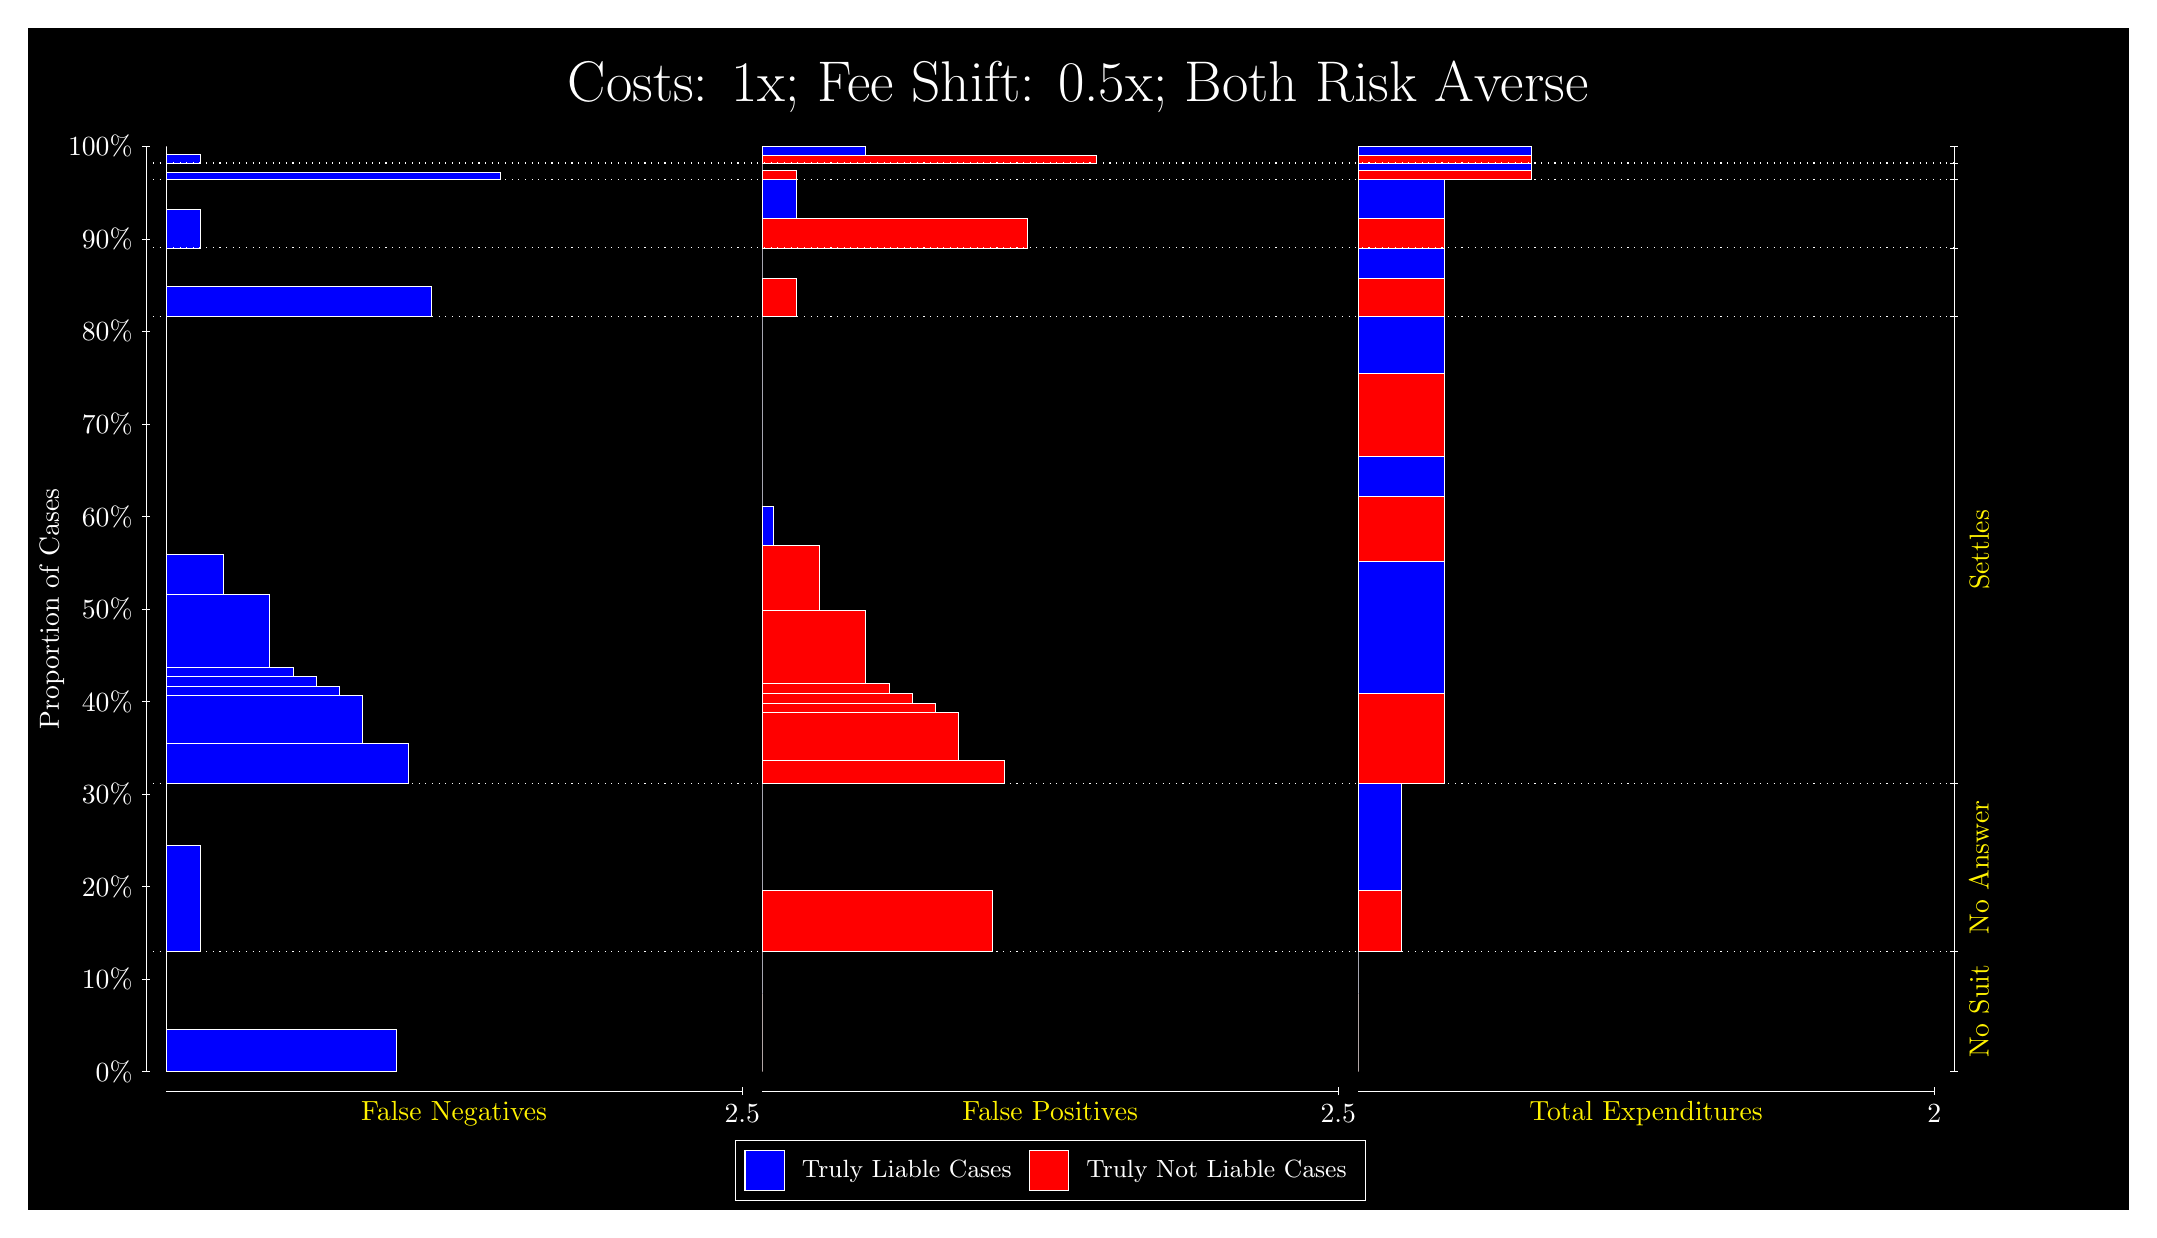
\begin{tikzpicture}
\draw[fill=black] (0,0) rectangle (26.667,15);
\draw[text=white] (0,13.5) rectangle (26.667,15) node[midway] {\huge Costs: 1x; Fee Shift: 0.5x; Both Risk Averse};
\draw[white, very thin] (1.5,1.75) -- (1.5,13.5);
\node[rotate=90, text=white, anchor=center] at (0.3, 7.625) {Proportion of Cases};
\draw[white, very thin] (1.45,1.75) -- (1.55,1.75);
\node[text=white, anchor=east] at (1.45, 1.75) {0\%};
\draw[white, very thin] (1.45,2.925) -- (1.55,2.925);
\node[text=white, anchor=east] at (1.45, 2.925) {10\%};
\draw[white, very thin] (1.45,4.1) -- (1.55,4.1);
\node[text=white, anchor=east] at (1.45, 4.1) {20\%};
\draw[white, very thin] (1.45,5.275) -- (1.55,5.275);
\node[text=white, anchor=east] at (1.45, 5.275) {30\%};
\draw[white, very thin] (1.45,6.45) -- (1.55,6.45);
\node[text=white, anchor=east] at (1.45, 6.45) {40\%};
\draw[white, very thin] (1.45,7.625) -- (1.55,7.625);
\node[text=white, anchor=east] at (1.45, 7.625) {50\%};
\draw[white, very thin] (1.45,8.8) -- (1.55,8.8);
\node[text=white, anchor=east] at (1.45, 8.8) {60\%};
\draw[white, very thin] (1.45,9.975) -- (1.55,9.975);
\node[text=white, anchor=east] at (1.45, 9.975) {70\%};
\draw[white, very thin] (1.45,11.15) -- (1.55,11.15);
\node[text=white, anchor=east] at (1.45, 11.15) {80\%};
\draw[white, very thin] (1.45,12.325) -- (1.55,12.325);
\node[text=white, anchor=east] at (1.45, 12.325) {90\%};
\draw[white, very thin] (1.45,13.5) -- (1.55,13.5);
\node[text=white, anchor=east] at (1.45, 13.5) {100\%};

\draw[white, very thin] (24.457,1.75) -- (24.457,13.5);
\draw[white, very thin] (24.407,1.75) -- (24.507,1.75);
\node[anchor=west] at (24.407, 1.75) {};
\draw[white, very thin] (24.407,3.2768) -- (24.507,3.2768);
\node[anchor=west] at (24.407, 3.2768) {};
\draw[white, very thin] (24.407,5.4074) -- (24.507,5.4074);
\node[anchor=west] at (24.407, 5.4074) {};
\draw[white, very thin] (24.407,11.342) -- (24.507,11.342);
\node[anchor=west] at (24.407, 11.342) {};
\draw[white, very thin] (24.407,12.21) -- (24.507,12.21);
\node[anchor=west] at (24.407, 12.21) {};
\draw[white, very thin] (24.407,13.077) -- (24.507,13.077);
\node[anchor=west] at (24.407, 13.077) {};
\draw[white, very thin] (24.407,13.288) -- (24.507,13.288);
\node[anchor=west] at (24.407, 13.288) {};
\draw[white, very thin] (24.407,13.5) -- (24.507,13.5);
\node[anchor=west] at (24.407, 13.5) {};

\draw[white, very thin, fill=blue] (1.75,1.75) rectangle (4.6775,2.2881);
\draw[white, very thin, fill=red] (1.75,2.2881) rectangle (1.75,3.2768);
\draw[white, very thin, fill=blue] (1.75,3.2768) rectangle (2.1891,4.6264);
\draw[white, very thin, fill=red] (1.75,4.6264) rectangle (1.75,5.4074);
\draw[white, very thin, fill=blue] (1.75,5.4074) rectangle (4.8239,5.9162);
\draw[white, very thin, fill=blue] (1.75,5.9162) rectangle (4.2384,6.5302);
\draw[white, very thin, fill=blue] (1.75,6.5302) rectangle (3.9457,6.6387);
\draw[white, very thin, fill=blue] (1.75,6.6387) rectangle (3.6529,6.7653);
\draw[white, very thin, fill=blue] (1.75,6.7653) rectangle (3.3602,6.8865);
\draw[white, very thin, fill=blue] (1.75,6.8865) rectangle (3.0674,7.815);
\draw[white, very thin, fill=blue] (1.75,7.815) rectangle (2.4819,8.3158);
\draw[white, very thin, fill=red] (1.75,8.3158) rectangle (1.75,11.342);
\draw[white, very thin, fill=blue] (1.75,11.342) rectangle (5.1167,11.722);
\draw[white, very thin, fill=red] (1.75,11.722) rectangle (1.75,12.21);
\draw[white, very thin, fill=blue] (1.75,12.21) rectangle (2.1891,12.697);
\draw[white, very thin, fill=red] (1.75,12.697) rectangle (1.75,13.077);
\draw[white, very thin, fill=blue] (1.75,13.077) rectangle (5.9949,13.173);
\draw[white, very thin, fill=red] (1.75,13.173) rectangle (1.75,13.288);
\draw[white, very thin, fill=blue] (1.75,13.288) rectangle (2.1891,13.404);
\draw[white, very thin, fill=red] (1.75,13.404) rectangle (1.75,13.5);
\draw[white, very thin, fill=red] (9.3189,1.75) rectangle (9.3189,2.7387);
\draw[white, very thin, fill=blue] (9.3189,2.7387) rectangle (9.3189,3.2768);
\draw[white, very thin, fill=red] (9.3189,3.2768) rectangle (12.246,4.0578);
\draw[white, very thin, fill=blue] (9.3189,4.0578) rectangle (9.3189,5.4074);
\draw[white, very thin, fill=red] (9.3189,5.4074) rectangle (12.393,5.7048);
\draw[white, very thin, fill=red] (9.3189,5.7048) rectangle (11.807,6.3187);
\draw[white, very thin, fill=red] (9.3189,6.3187) rectangle (11.515,6.4272);
\draw[white, very thin, fill=red] (9.3189,6.4272) rectangle (11.222,6.5538);
\draw[white, very thin, fill=red] (9.3189,6.5538) rectangle (10.929,6.675);
\draw[white, very thin, fill=red] (9.3189,6.675) rectangle (10.636,7.6036);
\draw[white, very thin, fill=red] (9.3189,7.6036) rectangle (10.051,8.4338);
\draw[white, very thin, fill=blue] (9.3189,8.4338) rectangle (9.4652,8.9345);
\draw[white, very thin, fill=blue] (9.3189,8.9345) rectangle (9.3189,11.342);
\draw[white, very thin, fill=red] (9.3189,11.342) rectangle (9.758,11.829);
\draw[white, very thin, fill=blue] (9.3189,11.829) rectangle (9.3189,12.21);
\draw[white, very thin, fill=red] (9.3189,12.21) rectangle (12.686,12.59);
\draw[white, very thin, fill=blue] (9.3189,12.59) rectangle (9.758,13.077);
\draw[white, very thin, fill=red] (9.3189,13.077) rectangle (9.758,13.193);
\draw[white, very thin, fill=blue] (9.3189,13.193) rectangle (9.3189,13.288);
\draw[white, very thin, fill=red] (9.3189,13.288) rectangle (13.564,13.384);
\draw[white, very thin, fill=blue] (9.3189,13.384) rectangle (10.636,13.5);
\draw[white, very thin, fill=red] (16.888,1.75) rectangle (16.888,2.7387);
\draw[white, very thin, fill=blue] (16.888,2.7387) rectangle (16.888,3.2768);
\draw[white, very thin, fill=red] (16.888,3.2768) rectangle (17.437,4.0578);
\draw[white, very thin, fill=blue] (16.888,4.0578) rectangle (17.437,5.4074);
\draw[white, very thin, fill=red] (16.888,5.4074) rectangle (17.986,6.5538);
\draw[white, very thin, fill=blue] (16.888,6.5538) rectangle (17.986,8.2308);
\draw[white, very thin, fill=red] (16.888,8.2308) rectangle (17.986,9.061);
\draw[white, very thin, fill=blue] (16.888,9.061) rectangle (17.986,9.5699);
\draw[white, very thin, fill=red] (16.888,9.5699) rectangle (17.986,10.62);
\draw[white, very thin, fill=blue] (16.888,10.62) rectangle (17.986,11.342);
\draw[white, very thin, fill=red] (16.888,11.342) rectangle (17.986,11.829);
\draw[white, very thin, fill=blue] (16.888,11.829) rectangle (17.986,12.21);
\draw[white, very thin, fill=red] (16.888,12.21) rectangle (17.986,12.59);
\draw[white, very thin, fill=blue] (16.888,12.59) rectangle (17.986,13.077);
\draw[white, very thin, fill=red] (16.888,13.077) rectangle (19.083,13.193);
\draw[white, very thin, fill=blue] (16.888,13.193) rectangle (19.083,13.288);
\draw[white, very thin, fill=red] (16.888,13.288) rectangle (19.083,13.384);
\draw[white, very thin, fill=blue] (16.888,13.384) rectangle (19.083,13.5);
\draw[white, dotted] (1.5,3.2768) -- (24.457,3.2768);
\draw[white, dotted] (1.5,5.4074) -- (24.457,5.4074);
\draw[white, dotted] (1.5,11.342) -- (24.457,11.342);
\draw[white, dotted] (1.5,12.21) -- (24.457,12.21);
\draw[white, dotted] (1.5,13.077) -- (24.457,13.077);
\draw[white, dotted] (1.5,13.288) -- (24.457,13.288);
\draw[white, very thin] (1.75,1.5) -- (9.0689,1.5);
\node[text=yellow, anchor=north] at (5.4094, 1.5) {False Negatives};
\draw[white, very thin] (9.0689,1.45) -- (9.0689,1.55);
\node[text=white, anchor=north] at (9.0689, 1.45) {2.5};

\draw[white, very thin] (9.3189,1.5) -- (16.638,1.5);
\node[text=yellow, anchor=north] at (12.978, 1.5) {False Positives};
\draw[white, very thin] (16.638,1.45) -- (16.638,1.55);
\node[text=white, anchor=north] at (16.638, 1.45) {2.5};

\draw[white, very thin] (16.888,1.5) -- (24.207,1.5);
\node[text=yellow, anchor=north] at (20.547, 1.5) {Total Expenditures};
\draw[white, very thin] (24.207,1.45) -- (24.207,1.55);
\node[text=white, anchor=north] at (24.207, 1.45) {2};

\node[text=yellow, centered, rotate=90] at (24.777, 2.5134) {No Suit};
\node[text=yellow, centered, rotate=90] at (24.777, 4.3421) {No Answer};
\node[text=yellow, centered, rotate=90] at (24.777, 8.3748) {Settles};





\draw (12.978300999999998,1.5) node[draw=none] (baseCoordinate) {};
\begin{scope}[align=center]
        \matrix[scale=0.5, draw=white, below=0.5cm of baseCoordinate, nodes={draw}, column sep=0.1cm]{
            \node[rectangle, draw, minimum width=0.5cm, minimum height=0.5cm, fill=blue] {}; &
            \node[draw=none, font=\small, text=white] (B) {Truly Liable Cases}; &
            \node[rectangle, draw, minimum width=0.5cm, minimum height=0.5cm, fill=red] {}; &
            \node[draw=none, font=\small, text=white] (B) {Truly Not Liable Cases}; \\
            };
\end{scope}

\end{tikzpicture}
\end{document}